\chapter{Træer}
\section{Terminologi for træer}

Sammenhængende grafer, der ikke indeholder en simpel kreds, kaldes træer. Træer har anvendelser i en del forskellige algoritmer.

\begin{defn}
Et træ er en sammenhængende ikke-orienteret graf, der ikke indeholder en simpel kreds.
\label{def_tree}
\end{defn}

Træer er en type af simple grafer. Da de ikke indeholder en simpel kreds, kan der ikke være flere kanter mellem to knuder, og der kan ikke være løkker. Alternativt og ækvivalent til Definition \ref{def_tree} gælder følgende om et træ.

\begin{thm}\label{thm:vej_tree}
En ikke-orienteret graf er et træ hvis og kun hvis, der eksisterer netop én simpel vej mellem hvert par af knuder. 
\end{thm}

\begin{proof}
	Antag at en ikke-orienteret graf, $T$, er et træ, og lad $u$ og $v$ være to knuder i $T$. 
	Da $T$ er sammenhængende må det betyde, at der er en simpel vej mellem $u$ og $v$ jf. Sætning \ref{smh_satning}. 
	Den simple vej mellem $u$ og $v$ må være den eneste vej mellem $u$ og $v$, for hvis der eksisterer flere veje mellem $u$ og $v$, eksisterer en simpel kreds. 
	Antag for modstrid, at der mellem $u$ og $v$ er to forskellige simple veje $P_{u,v}$ og $P_{v,u}$. Da må der være mindst ét punkt, der er forskelligt mellem de to veje. 
	En simpel kreds opstår fra og med knuden $x$, hvor $P_{u,v}$ og $P_{v,u}$ første gang adskiller sig fra hinanden. 
	Den simple kreds slutter, når $P_{u,v}$ og $P_{v,u}$ igen har en knude $y$ til fælles og består derfor af knuderne mellem $x$ og $y$ i begge veje.
	Eksistensen af en simpel kreds modstrider antagelsen om, at $T$ er et træ, og derfor må der være netop én simpel vej mellem hvert knudepar i $T$.

Antag nu, at der er netop én simpel vej mellem hvert knudepar i en ikke-orienteret graf $T$.
	Det betyder, at $T$ er sammenhængende. Desuden må det gælde, at $T$ ingen simple kredse har, da det vil stride i mod antagelsen om, at der er netop én simpel vej mellem hvert knudepar i $T$.
	Der kan ikke eksistere en simpel kreds, da der kun er én simpel vej mellem to knuder $u$ og $v$. Derfor kan der ikke findes knuder, hvor to eller flere veje mellem $u$ og $v$ adskiller fra hinanden, hvor der kan dannes en kreds.
	Grafen $T$ opfylder dermed kravene for at være et træ jf. Definition \ref{def_tree}.
\end{proof}

\begin{exmp}
For at illustrere en graf, som er et træ, og en graf, som ikke er et træ, iagttages hhv. Figur \ref{eksempel_tree} og Figur \ref{eksempel_notree}. Grafen i Figur \ref{eksempel_tree} er et træ, da det er en ikke-orienteret sammenhængende graf uden simple kredse.

Grafen i Figur \ref{eksempel_notree} er ikke et træ, da der eksistrer en kreds $\lbrace B, D, C, B \rbrace$. 
Et andet argument for, at grafen ikke er et træ, er, at grafen ikke er sammenhængende.
\end{exmp}

\begin{figure}[h]
\centering
	\begin{subfigure}{0.5\textwidth}
		\centering
			\scalebox{0.9}{\input{fig/tikz/et_trae}}
		\caption{Et træ.} 
		\label{eksempel_tree}
	\end{subfigure}%
	\begin{subfigure}{0.5\textwidth}
		\centering		
			\scalebox{0.9}{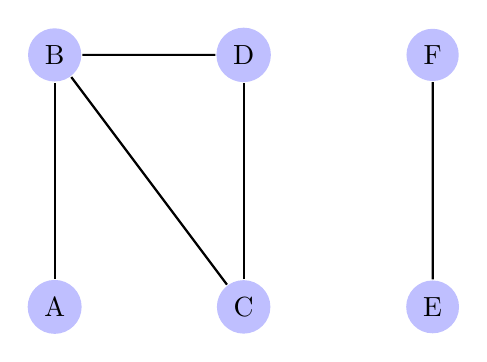
\begin{tikzpicture}
[thick,scale=.8,auto=left,every node/.style={circle,fill=blue!25}]
  \node (n6) at (3,2) {A};
  \node (n4) at (3,6) {B};
  \node (n5) at (6,2) {C};
  \node (n1) at (6,6) {D};
  \node (n2) at (9,2) {E};
  \node (n3) at (9,6) {F};
  \foreach \from/\to in {n6/n4,n4/n5,n5/n1,n2/n3,n4/n1}
    \draw (\from) -- (\to);
\end{tikzpicture}}
		\caption{En graf, der ikke er et træ.} 
		\label{eksempel_notree}
	\end{subfigure}
\caption{}
\end{figure}

\section{Udspændende træer}

Et udspændende træ er et træ, der indeholder alle knuder i en simpel, sammenhængende graf.

\begin{defn}
I en simpel graf, $G$, er et udspændende træ en delgraf af $G$, der indeholder alle knuder i $G$, og som opfylder betingelserne for at være et træ.
\end{defn}

En simpel graf med et udspændende træ er sammenhængende, fordi der er en vej mellem alle knuder i det udspændende træ.
Det omvendte gælder også dvs. at hver simpel sammenhængende graf har et udspændende træ, hvilket kan formuleres i det følgende.

\begin{thm}
En simpel graf er sammenhængende hvis og kun hvis, den har et udspændende træ.
\end{thm}

\begin{proof}
Først antages det, at en simpel graf, $G$, har et udspændende træ. 
Træet $T$ indeholder alle knuder i $G$ og har en simpel vej mellem alle knudepar, fordi $T$ er et træ. 
Fordi $T$ er en delgraf af $G$, så er der en vej mellem alle knuder i $G$, og derfor er $G$ sammenhængende.

Det antages nu, at $G$ er sammenhængende. Hvis $G$ ikke er et træ, så indeholder den mindst en simpel kreds. 
Der fjernes nu en kant i en af de simple kredse. 
Resultatet er en delgraf af $G$, der har en kant mindre end $G$, og som stadig indeholder alle knuder i $G$ og stadig er sammenhængende. 
Grafen er stadig sammenhængende, fordi knuderne, der var forbunde af den fjernede kant, stadig er forbundne af en vej, der ikke indeholder den fjernede kant, fordi den fjernede kant var en del af en simpel kreds. 
Er der flere simple kredse, gentages processen med at fjerne kanter for at eliminere simple kredse, indtil der ikke er flere. 
Resultatet er et træ, fordi $G$ forbliver sammenhængende, i takt med kanter fjernes. Træet er et udspændende træ, fordi det stadig indeholder alle knuder i $G$.
\end{proof}

\begin{exmp}
Betragt grafen i Figur \ref{eksempel_udspaendende}. Grafen er simpel og sammenhængende, og derfor kan der findes et udspændende træ. 

\begin{figure}[h]
\centering
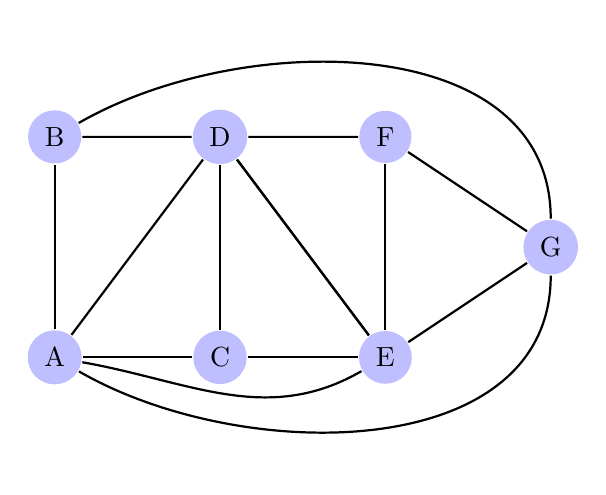
\begin{tikzpicture}
[thick,scale=.7,auto=left,every node/.style={circle,fill=blue!25}]
  \node (n6) at (3,2) {A};
  \node (n4) at (3,6) {B};
  \node (n5) at (6,2) {C};
  \node (n1) at (6,6) {D};
  \node (n2) at (9,2) {E};
  \node (n3) at (9,6) {F};
  \node (n7) at (12,4) {G};
  \foreach \from/\to in {n6/n4,n5/n1,n2/n3,n4/n1,n6/n1,n1/n2,n3/n7,n7/n2,n5/n6,n5/n2,n1/n2,n1/n3}
    \draw (\from) -- (\to);
    \draw (n4) to[out=30,in=90] (n7);
    \draw (n6) to[out=-10,in=-150] (n2);
    \draw (n6) to[out=-30,in=-90] (n7);
\end{tikzpicture}
\caption{En simpel sammenhængende graf} 
\label{eksempel_udspaendende}
\end{figure}

Der er mange muligheder for at finde et udspændende træ i grafen i Figur \ref{eksempel_udspaendende}. For at finde et udspændende træ, fjernes kanter i de simple kredse, indtil der opstår en sammenhængende undergraf, der indeholder alle knuderne i grafen. To eksempler på udspændende træer ses i Figur \ref{eksempel_udspaendende1}.

%Billede med 4 udspændende træer
\begin{figure}[!htb]
	\centering
	\begin{minipage}[c]{0.45\linewidth}
		\centering
		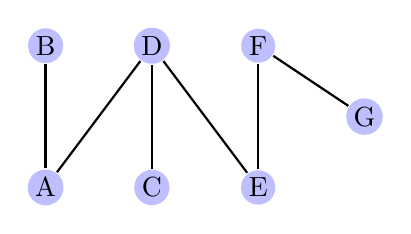
\begin{tikzpicture}[thick,scale=.45,auto=left,every node/.style={circle,fill=blue!25},inner sep=1pt,minimum size=2pt]
		  \node (n6) at (3,2) {A};
		  \node (n4) at (3,6) {B};
		  \node (n5) at (6,2) {C};
		  \node (n1) at (6,6) {D};
		  \node (n2) at (9,2) {E};
		  \node (n3) at (9,6) {F};
		  \node (n7) at (12,4) {G};
		  \foreach \from/\to in {n6/n4,n6/n1,n1/n5,n1/n2,n2/n3,n3/n7}
		    \draw (\from) -- (\to);
		\end{tikzpicture}
	\end{minipage}
	\begin{minipage}[c]{.45\linewidth}
		\centering
		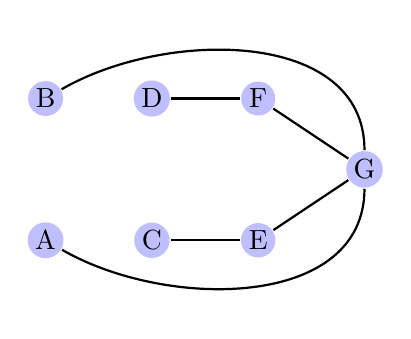
\begin{tikzpicture}[thick,scale=.45,auto=left,every node/.style={circle,fill=blue!25},inner sep=1pt,minimum size=2pt]
		  \node (n6) at (3,2) {A};
		  \node (n4) at (3,6) {B};
		  \node (n5) at (6,2) {C};
		  \node (n1) at (6,6) {D};
		  \node (n2) at (9,2) {E};
		  \node (n3) at (9,6) {F};
		  \node (n7) at (12,4) {G};
		  \foreach \from/\to in {n7/n3,n1/n3,n2/n5,n2/n7}
		    \draw (\from) -- (\to);
		    \draw (n4) to[out=30,in=90] (n7);
			\draw (n6) to[out=-30,in=-90] (n7);
		\end{tikzpicture}
	\end{minipage}
	\caption{To forskellige eksempler på udspændende træer på den samme graf.} \label{eksempel_udspaendende1}
\end{figure}

\end{exmp}

\section{Minimale udspændende træer}

En række problemer involverer at finde den eksempelvis korteste, billigste eller på anden vis mest favorable forbindelse, der inkluderer alle knuder i en vægtet graf. Problemet kan løses ved at bestemme et minimalt udspændende træ. I et minimalt udspændende træ er summen af kanternes vægt mindst mulig, og træet indeholder alle knuder i grafen.

\begin{defn}
Et minimalt udspændende træ i en sammenhængende vægtet graf er et udspændende træ, som har den mindst mulige sum af kanternes vægt.
\end{defn}

Der findes forskellige algoritmer til at finde minimale udspændende træer i vægtede grafer, hvor et eksempel er Prims algoritme, som ses i Algoritme \ref{find_mintrae}. 

\begin{algorithm}
\caption{Prims algoritme}
\label{find_mintrae}
\textbf{procedure} Prim($G$: En vægtet, sammenhængende, ikke-orienteret graf med $n$ knuder)

$T:=$ En kant med mindst mulig vægt\\
\textbf{for} $i:=1$ \textbf{til} $n-2$\\
$\-$ $\-$ $\-$ $\-$ $\-$ $\-$
$e:=$ En kant med mindst vægt incident til en knude i $T$, som ikke danner en simpel kreds, når den tilføjes $T$.\\
$\-$ $\-$ $\-$ $\-$ $\-$ $\-$
$T:=T$ hvor $e$ er tilføjet.\\
\textbf{retunér} $T$ $\lbrace T$ er et minimalt udspændende træ.$\rbrace$
\end{algorithm}

Prims algoritme er en grådig algoritme, der tager udgangspunkt i en kant med mindst mulig vægt. 
Ud fra kanten vælges en ny incident kant med mindst mulig vægt, så der ikke dannes en kreds ved tilføjelse af den nye kant. 
Dvs. at der ved hvert trin vælges kanten med den mindste vægt. 
Sammenlagt vil algoritmen finde den optimale løsning og dermed finde et minimalt udspændende træ. 
Der kan i Prims algoritme opstå, at algoritmen kan vælge mellem flere kanter med samme vægt, og der vil derfor kræves en form for rangering af kanterne. 

Desuden er Prims algoritme anvendelig, idet den er af polynomiel kompleksitet.

\begin{thm}
	Prims algoritme har tidskompleksiteten $O (n^3)$.
	\label{prim_kompl}
\end{thm}
\begin{proof}
	For at bestemme tidskompleksiteten skal der findes det værst mulige antal af skridt, algoritmen udfører.
	Der tages udgangspunkt i antallet af sammenligninger, algoritmen foretager.
	For simple grafer er en komplet graf den graf, der har flest mulige kanter og vil derfor være den værst mulige graf i forhold til antallet af sammenligninger, algoritmen foretager.

	I starten består træet, $T$, af to naboknuder, hvilket også betyder, at antallet af knuder, $n$, må være større end $1$.
	Derefter vil der for hver knude i $T$, $t_j$, laves en sammenligning med hver knude i grafen, der ikke er i $T$, $t_k$, for at finde ud af, om den foreløbige mindste vægt for $t_j$ og en naboknude er større end $d(t_j, t_k)$.
	Antallet af skridt, mens der er to knuder i $T$ for at tilføje en ny knude til $T$, må da være $2 \cdot (n - 2)$.
	Derefter er der tre knuder i $T$, og antallet af sammenligninger for at tilføje endnu en knude må nu være $3 \cdot (n - 3)$.
	Når der kun er én knude tilbage, der ikke er i $T$, laves der kun $(n-1)$ sammenligninger.
	Da må det samlede antal af sammenligninger, $f(n)$, være
	\begin{align*}
		f(n) = 2 (n-2) + 3(n-3) + \dotsb + (n-3) 3 + (n-2) 2 + (n -1).
	\end{align*}
	Der er $n -2$ led i denne sum. Værdien $n-2$ er større end både $n-3, n-4, ..., 1$ når $n > 1$ og da må
	\begin{align*}
		f(n)
		&\leq 2 (n-2) + 3 (n-2) + \dotsb + (n-2) (n-2) + (n-1) (n-2) \\
		&= (n-2) \left( 2 + 3 + \dotsb + (n-2) + (n-1) \right) \\
		&= (n-2) \left( \frac{n(n-1)}{2} - 1 \right) \\
		&= \frac{1}{2} n^3 - \frac{1}{2} n^2 - 2n + 2 \\
		&\leq 2n^3 - n^3 - 2n^3 + 2n^3 \\
		&= n^3,
	\end{align*}
	når $n > 1$. Her er vidnerne $k=1$ og $C=1$, og da må $f(n)$ være $O(n^3)$.
\end{proof}


\begin{figure}[!h]
  \centering
  \scalebox{0.8}{\begin{tikzpicture}
  [shorten >=1pt,node distance=3.1cm,on grid,auto]
    \tikzstyle{state}=[shape=circle,fill=blue!25,thick,minimum size=0.7cm]

    \node[state] (G) {$G$};
    \node[state,above of=G] (D) {$D$};
    \node[state,right of=G] (H) {$H$};
    \node[state,right of=D] (E) {$E$};
    \node[state,right of=H] (I) {$I$};
    \node[state,right of=E] (F) {$F$};
    \node[state,above of=D] (A) {$A$};
    \node[state,right of=A] (B) {$B$};
    \node[state,right of=B] (C) {$C$};

    \path[-,draw,thick]
    (G) edge node {$6$} (D);
    \path[-,draw,thick,red]
    (D) edge node {$2$} (A)
    (E) edge node {$3$} (H)
    (H) edge node {$2$} (I)
    (E) edge node {$1$} (F);
    \path[-,draw,thick]
    (I) edge node {$4$} (F);
    \path[-,draw,thick,red]  
    (G) edge node {$4$} (H);
    \path[-,draw,thick]
    (A) edge node {$5$} (B);
    \path[-,draw,thick,red]
    (B) edge node {$4$} (C);
    \path[-,draw,thick]
    (D) edge node {$7$} (E)  
    (B) edge node {$5$} (E);
    \path[-,draw,thick,red]
    (C) edge node {$3$} (F);
    \path[-,draw,thick]
    (B) edge node {$6$} (F);
    \path[-,draw,thick,red]
    (D) edge node {$3$} (B);
    \path[-,draw,thick]
    (D) edge node {$8$} (H)
    (H) edge node {$4$} (F)
    ;
  \end{tikzpicture}}
  \caption{Eksempel på et minimalt udspændende træ.}
  \label{eks_prim}
\end{figure}

\begin{exmp}
For at give et eksempel på princippet i Prims algoritme laves et eksempel på at finde et minimalt udspændende træ i grafen i Figur \ref{eks_prim}. 
Prims algoritme vil i første skridt vælge en kant med mindst mulig vægt. 
I grafen vil det være $\lbrace E,F \rbrace$ med vægt $1$. 
Næste skridt vil være at vælge en kant incident med $E$ eller $F$ med mindst mulig vægt. 
Der kan vælges $\lbrace C,F \rbrace$ eller $\lbrace E,H \rbrace$ alt efter hviken rangering af kanter med samme vægt, der vælges. 
Der vælges kanten $\lbrace C,F \rbrace$. 
Næste skridt vil være at vælge en kant incident med $E$, $F$ eller $C$ med mindst mulig vægt, uden at der dannes en simpel kreds med de allerede valgte kanter. 
Der vælges $\lbrace E,H \rbrace$. Dernæst vælges $\lbrace H,I \rbrace$. 
Der kan nu vælges enten $\lbrace B,C \rbrace$  eller $\lbrace G,H \rbrace$ med vægt 4. 
Der vælges $\lbrace G,H \rbrace$ efterfulgt af $\lbrace B,C \rbrace$. 
Der vælges nu $\lbrace B,D \rbrace$ efterfulgt af $\lbrace A,D \rbrace$.

Alle knuder er nu besøgt, og der er dermed dannet et minimalt udspændende træ med kanterne $\lbrace E,F \rbrace$, $\lbrace C,F \rbrace$, $\lbrace E,H \rbrace$, $\lbrace H,I \rbrace$, $\lbrace G,H \rbrace$, $\lbrace B,C \rbrace$, $\lbrace B,D \rbrace$, $\lbrace A,D \rbrace$. 
Alt efter rangering af kanter med samme vægt kan rækkefølgen, algoritmen vælger kanter, variere, men der opnås i dette eksempel samme minimale udspændende træ.
\end{exmp} 

Det vil med udgangspunkt i \citep{prim} bevises, at Prims algoritme bestemmer et minimalt udspændende træ.

\begin{thm}
Prims algoritme bestemmer et minimalt udspændende træ. 
\label{set_prim}
\end{thm}


%\begin{proof}
%Lad $G$ være en sammenhængende vægtet graf. Lad $S$ være træet bestående af $e_1$, $e_2$, $\ldots$, $e_{n-1}$ valgt af Prims algoritme. Lad $T$ være et minimalt udspændende træ i $G$ bestående af kanterne $e_1$, $e_2$, $\ldots$, $e_k$, hvor $k$ er det maksimale antal kanter, så $T$ stadig er et minimalt udspændende træ. I følge Sætning \ref{set_prim} skal $S=T$. 

%Det antages for modstrid, at $S \neq T$, således at, $k<n-1$. Det betyder, at der er i $T$ er færre kanter end i $S$, og $T$ består derfor af $e_1$, $e_2$, $\ldots$, $e_k$ men ikke $e_{k+1}$. 
%Lad $S_k$ være træet valgt af Prim algortime bestående af $e_1$, $e_2$, $\ldots$, $e_k$. Antag nu, at der dannes en graf bestående af $T$, hvor $e_{k+1}$ tilføjes. 
%Da der tilføjes en kant til et udspændende træ, dannes der en kreds, som må indeholde $e_{k+1}$, da $e_{k+1}$ ikke er en del af $T$. 
%Algoritmen vil aldrig danne en kreds i $S_{k+1}$, derfor må der findes en anden kant $e$ i kredsen som ikke er del af $S_{k+1}$.
%Kanten $e$ fjernes fra T, og $e_{k+1}$ tilføjes, og der dannes et nyt træ $T'$  
%Fordi $e_{k+1}$ er valgt af Prims algoritme, mens $e$ også var tilgængelig, må $e_k{k+1}$ have mindre eller samme vægt som $e$. 
%Det betyder at $T'$ også er et minimalt udspændende træ. 

%\end{proof}


\begin{proof}
Lad $T_{k}$ være et træ. Det skal så med induktion vises, at $T_{k}$, som tilføjes en kant, $e$, er et undertræ af et minimalt udspændende træ, $M$. 

\textit{Basisskridt}: Da $T_0$ i begyndelsen blot består af en enkelt knude uden kanter, må den være et undertræ af $M$.

\textit{Induktionsskridtet}: Ved $k$'te skridt i algoritmen, er $T_k$ et undertræ af $M$, og Prims algoritme tilføjer kanten $e$. Hvis $e$ $\in$ $M$, må $T_k$ stadig være et undertræ af $M$ i følge induktionsantagelsen.

Antag for modstrid, at $e \notin M$. Når $e$ tilføjes $M$, dannes der netop én kreds, fordi $M$ er et udspændende træ og derfor har én simpel vej mellem alle knuder jf. Sætning \ref{thm:vej_tree}.
Kanten $e$ har en endeknude i $T_k$ samt en endeknude, der ikke er i $T_k$, fordi Prims algoritme har tilføjet $e$. 
Der vil eksistere en anden kant $e'$ i kredsen, som også har netop en endeknude i $T_k$, fordi $e$ skal have endeknude i $M$, uden at $e$ er del af $M$. 
Kanterne $e$ og $e'$ er illustreret i Figur \ref{graf_prim_bevis}, hvor det kan ses, at de er en del af en kreds. 
Prims algoritme kunne have valgt $e'$, men valgte at tilføje $e$, hvorfor $d(e) \leq d(e')$. 
Hvis $e$ tilføjes til $M$, mens $e'$ fjernes fra samme kreds, opstår et nyt træ $M'$, hvor 
$d(M') \leq d(M)$, hvilket er i modstrid med, at $M$ er et minimalt udspændende træ. Det nye træ $M'$ indeholder $T_k\cup \lbrace e \rbrace$, hvilket følger induktionsantagelsen. 
\end{proof}

\begin{figure}[h]
\centering
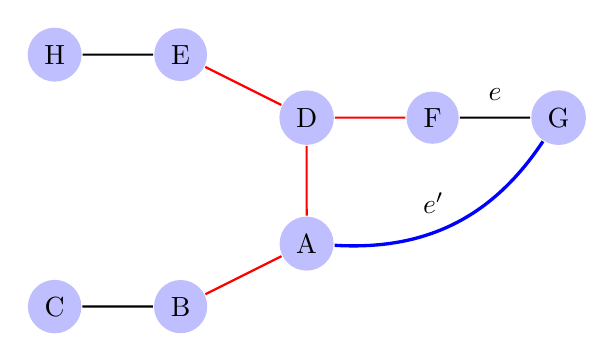
\begin{tikzpicture}
[thick,scale=.8,auto=left,every node/.style={circle,fill=blue!25}]
  \node (n6) at (4,4) {A};
  \node (n4) at (2,3) {B};
  \node (n5) at (0,3) {C};
  \node (n1) at (4,6) {D};
  \node (n2) at (2,7) {E};
  \node (n3) at (6,6) {F};
  \node (n7) at (8,6) {G};
  \node (n8) at (0,7) {H};
  \foreach \from/\to in {n5/n4,n2/n8}
    \draw (\from) -- (\to);
    
  \path[-,draw,thick,red]
  	(n4) edge (n6)
  	(n6) edge (n1)
  	(n1) edge (n2)
  	(n1) edge (n3);
  \path[-,draw,black]
  	(n3) edge node[draw=none,fill=none] {$e$} (n7);
  \path[-,draw,very thick,blue,bend right]
  	(n6) edge node[draw=none,fill=none,color=black] {$e'$} (n7);
\end{tikzpicture}
\caption{Graf til beviset for Prims algoritme. Den røde del af grafen udgør $T_k$, og den røde og sorte del udgør tilsammen $M$.  } 
\label{graf_prim_bevis}
\end{figure}
